% !TEX root = ../discretemath.tex

\section{Диаграммы Юнга и производящие функции на них}

\subsection{Разбиения и диаграммы Юнга}

\begin{Definition}{Разбиение / диаграмма Юнга}{}
	\emph{Разбиение} числа $n$ — невозрастающая последовательность $\lambda=(\lambda_1\ge\lambda_2\ge\dots\ge\lambda_k>0)$ с $\sum_i\lambda_i=n$. Число $|\lambda|=n$ — \emph{вес}, $\lambda_i$ — \emph{части}. \emph{Диаграмма Юнга} — $n$ клеток в строках: $i$-я строка содержит $\lambda_i$ клеток (выровнены влево, сверху вниз).
\end{Definition}

\begin{Example}{}{}
	$\lambda=(6,6,3,1,1)$, вес $|\lambda|=17$.
	\begin{center}
		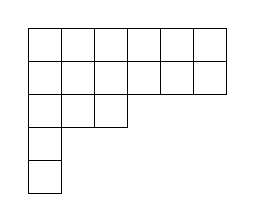
\begin{tikzpicture}[scale=0.42]
			\foreach \col in {1,...,6} { \draw (\col-1,4) rectangle (\col,5); }
			\foreach \col in {1,...,6} { \draw (\col-1,3) rectangle (\col,4); }
			\foreach \col in {1,...,3} { \draw (\col-1,2) rectangle (\col,3); }
			\draw (0,1) rectangle (1,2);
			\draw (0,0) rectangle (1,1);
		\end{tikzpicture}
	\end{center}
	Три записи: убывающая $(6,6,3,1,1,0,\dots)$; экспоненциальная $1^2\cdot 3^1\cdot 6^2$; частотная $(m_1,m_2,\dots)=(2,0,1,0,0,2,0,\dots)$, где $m_k=\#\{i:\lambda_i=k\}$.
\end{Example}

\subsection{Производящая функция для разбиений}

Производящая функция по всем диаграммам Юнга (включая пустую):
\[
F(q)=\sum_{\lambda}q^{|\lambda|}=1+q+2q^2+3q^3+5q^4+\cdots
\]

\begin{Theorem}{}{}
	\[
	F(q)=\prod_{k=1}^{\infty}\frac{1}{1-q^k}.
	\]
\end{Theorem}

\begin{proof}
	Раскроем каждый множитель в геометрический ряд:
	\[
	\prod_{k=1}^{\infty}\frac{1}{1-q^k}=\prod_{k=1}^{\infty}\bigl(1+q^k+q^{2k}+\cdots\bigr).
	\]
	При раскрытии скобок выбор показателя $m_k\ge 0$ в $k$-м множителе означает «часть размера $k$ встречается $m_k$ раз» и даёт вклад $q^{\sum_k k m_k}=q^{|\lambda|}$. Суммирование по всем выборам $(m_k)$ — это суммирование по всем диаграммам Юнга, откуда $F(q)$.
\end{proof}

\subsection{Уточнённые производящие функции}

\begin{Theorem}{}{}
	При фиксированном $n\ge 1$:
	\[
	\sum_{\substack{\lambda:\ \text{все части}\le n}}q^{|\lambda|}
	=\sum_{\substack{\lambda:\ \text{не более }n\text{ строк}}}q^{|\lambda|}
	=\prod_{k=1}^{n}\frac{1}{1-q^k}.
	\]
\end{Theorem}

Равенство двух сумм — биекция \emph{сопряжения}: $\lambda\mapsto\lambda^{T}$ (отражение по главной диагонали) переводит «все части $\le n$» в «не более $n$ строк». Равенство произведению — тот же аргумент, что в основной теореме, но с $k\in\{1,\dots,n\}$.

\begin{Theorem}{}{}
	\[
	\sum_{\substack{\lambda:\ \text{ровно }n\text{ строк}}}q^{|\lambda|}=q^n\prod_{k=1}^{n}\frac{1}{1-q^k}.
	\]
\end{Theorem}

\begin{proof}
	Если $\lambda$ имеет ровно $n$ строк ($\lambda_n\ge 1$), положим $\mu_i=\lambda_i-1$. Тогда $\mu$ — не более $n$ строк и $|\lambda|=|\mu|+n$, откуда множитель $q^n$ и сумма по $\mu$ (не более $n$ строк).
\end{proof}

\begin{Statement}{Двупараметрическое обобщение}{}
	С переменной $t$, отслеживающей число строк:
	\[
	\sum_{\lambda}t^{\#\mathrm{строк}(\lambda)}q^{|\lambda|}=\prod_{k=1}^{\infty}\frac{1}{1-tq^k}=\prod_{k=1}^{\infty}\bigl(1+tq^k+(tq^k)^2+\cdots\bigr).
	\]
\end{Statement}

\subsection{Разбиения с ограниченной кратностью}

Рассмотрим разбиения, в которых каждая часть встречается $0$ или $\ge 2$ раз (но не ровно $1$). Для каждого $k$ множитель: $1+q^{2k}+q^{3k}+\cdots$.

\begin{Theorem}{}{}
	\[
	G(q)=\prod_{k=1}^{\infty}\bigl(1+q^{2k}+q^{3k}+\cdots\bigr)=\prod_{k=1}^{\infty}\frac{1+q^{3k}}{1-q^{2k}}.
	\]
\end{Theorem}

\begin{proof}
	Для каждого $k$: $1+q^{2k}+q^{3k}+\cdots=\dfrac{1-q^k+q^{2k}}{1-q^k}$. Так как $(1+q^k)(1-q^k+q^{2k})=1+q^{3k}$ и $(1-q^k)(1+q^k)=1-q^{2k}$, получаем $\dfrac{1-q^k+q^{2k}}{1-q^k}=\dfrac{1+q^{3k}}{1-q^{2k}}$. Перемножая по всем $k$ — формула. (Комбинаторную биекцию найти сложнее, чем это алгебраическое тождество.)
\end{proof}
